\documentclass[10pt,xcolor=pdflatex]{beamer}
\usepackage{newcent}
\usepackage[utf8]{inputenc}
\usepackage[czech]{babel}
\usepackage{hyperref}
\usepackage{fancyvrb}
\usepackage{graphicx}
\usepackage{textpos}
\usepackage{tikz}
\usepackage{textcomp}
\usepackage[export]{adjustbox}
\usepackage{float}
\usepackage{alltt}
\usepackage{hyperref}
\usepackage{textpos}
\usepackage{multicol}
\usepackage{tikz}
\usepackage{fancyvrb}
\usepackage{color}
\usepackage{subfig}
\usepackage{geometry}
\usepackage{graphicx}
\usepackage{epstopdf}
\usepackage{multicol}
\usetheme{FIT}

\newcommand{\myuv}[1]{\quotedblbase #1\textquotedblleft}
\def\uv#1{\quotedblbase#1\textquotedblleft}%

%%%%%%%%%%%%%%%%%%%%%%%%%%%%%%%%%%%%%%%%%%%%%%%%%%%%%%%%%%%%%%%%%%
\title[GJA 3]{RMI and JMS}

\author[]{Jaroslav Dytrych}

\institute[]{Faculty of Information Technology
Brno University of Technology \\
Bo\v{z}et\v{e}chova 1/2. 612 66 Brno - Kr\'alovo Pole\\
dytrych@fit.vutbr.cz}

\date{2 October 2023}
%\date{\today}
%\date{} % bez data

%%%%%%%%%%%%%%%%%%%%%%%%%%%%%%%%%%%%%%%%%%%%%%%%%%%%%%%%%%%%%%%%%%

\begin{document}

\frame[plain]{\titlepage}

\begin{frame}\frametitle{Content}
\begin{itemize}
	\item RMI (Remote Method Invocation)
    \item JMS (Java Message Service)
\end{itemize}
\end{frame}


\bluepage{RMI (Remote Method Invocation)}

\begin{frame}[containsverbatim]\frametitle{RMI}
\begin{itemize}
	\item RMI
      \begin{itemize}
    	\item Remote method invocation
		\item Distributed Java
		\item TCP/IP transport layer
		\item Allow code that defines behavior and code that implements behavior to remain separate and to run on separate JVMs
		\item Part of JDK since Java 1.1
		\item Code running on one JVM may call method on other JVM
		\item Client/Server architecture
      \end{itemize}
\end{itemize}
\begin{tikzpicture}[remember picture,overlay]
    \node[xshift=-0.6cm,yshift=-1.3cm] at (current page.north east){%
    
\includegraphics[width=1cm]{img/oko}};
\end{tikzpicture}
\end{frame}


\begin{frame}[containsverbatim]\frametitle{RMI protocols}
\begin{itemize}
	\item RMI uses a protocol called Java Remote Method Protocol
	  \begin{itemize}
		\item JRMP is proprietary
	  \end{itemize}
    \item For increased interoperability RMI later used the Internet Inter-ORB Protocol (IIOP)
	  \begin{itemize}
		\item IIOP is CORBA's communication protocol using TCP/IP as the transport. CORBA is Common Object Request Broker Architecture
		\item language neutral protocol
		\item standard way to make method calls to remote objects
		\item \texttt{PortableRemoteObject} instead of \texttt{UnicastRemoteObject}
		\item \texttt{-iiop} parameter of the \texttt{rmic} compiler
		\item In JDK 11, the Java EE and CORBA modules were removed. These modules were deprecated for removal in JDK 9.
	  \end{itemize}
    \item RMI is all about remote calls at runtime.
	  \begin{itemize}
		\item It’s not about compilation against a remote class.
	  \end{itemize}
\end{itemize}
\end{frame}


\begin{frame}[containsverbatim]\frametitle{RMI architecture}
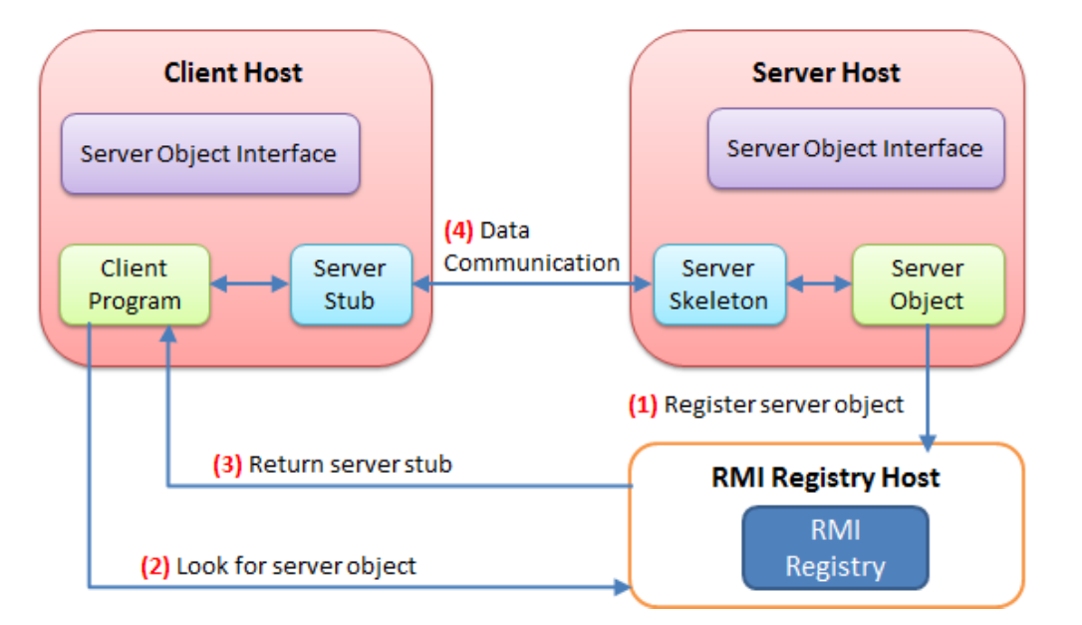
\includegraphics[scale=0.41]{img/obr1}
\begin{tikzpicture}[remember picture,overlay]
    \node[xshift=-0.6cm,yshift=-1.3cm] at (current page.north east){%
    
\includegraphics[width=0.8cm]{img/pozor}};
\end{tikzpicture}
\end{frame}


\begin{frame}[containsverbatim]\frametitle{RMI features}
\begin{itemize}
	\item Simplifies communication with remote applications
	  \begin{itemize}
		\item local method calls
	  \end{itemize}
    \item Supports security
	  \begin{itemize}
		\item on both server and client side
	  \end{itemize}
	\item RMI layers
      \begin{itemize}
    	\item Stub
          \begin{itemize}
            \item client side
            \item creates marshall stream from client requests
            \item demarshalling server response
            \item object references are accessible via stub
          \end{itemize}
        \item Skeleton 
          \begin{itemize}
            \item server side
            \item transforms marshall stream to method call
          \end{itemize}
      \end{itemize}
\end{itemize}
\begin{tikzpicture}[remember picture,overlay]
    \node[xshift=-0.6cm,yshift=-1.3cm] at (current page.north east){%
    
\includegraphics[width=1cm]{img/pozor}};
\end{tikzpicture}
\end{frame}


\begin{frame}[containsverbatim]\frametitle{RMI principles}
\begin{itemize}
	\item RMI uses proxy design pattern
	  \begin{itemize}
		\item An object in one context is represented by another (the~stub)~in a separate context.
		\item The stub knows how to forward method calls between the participating objects.
	  \end{itemize}
    \item A naming or directory service is run on a well-known host and port number
	  \begin{itemize}
		\item usually port 1099
	  \end{itemize}
    \item RMI includes RMI registry
	  \begin{itemize}
		\item which is actually a naming service
		\item may be created directly in java or by “\texttt{rmiregistry}” program available in JDK
	  \end{itemize}
    \item Stubs and skeletons are generated
	  \begin{itemize}
		\item Static stubs and skeletons can be created by \texttt{rmic} program 
		  \begin{itemize}
		      \item Deprecated
		  \end{itemize}
		\item Skeletons and stubs should be generated dynamically
		  \begin{itemize}
		      \item 5 ways, e.g. subclassing \texttt{UnicastRemoteObject} and calling it's constructor (\texttt{super()}).
		  \end{itemize}
	  \end{itemize}
\end{itemize}
\begin{tikzpicture}[remember picture,overlay]
    \node[xshift=-0.6cm,yshift=-1.3cm] at (current page.north east){%
    
\includegraphics[width=1cm]{img/pozor}};
\end{tikzpicture}
\end{frame}


\begin{frame}[containsverbatim]\frametitle{RMI Registry}
\begin{itemize}
  \item The RMI registry is a simple server-side bootstrap naming facility that enables remote clients to obtain a reference to an initial remote object. 
  \item It can be started with the \texttt{rmiregistry} command which produces no output and is typically run in the background.
  \item Before you execute \texttt{rmiregistry}, you must make sure that the shell in which you will run \texttt{rmiregistry} either has no CLASSPATH environment variable set or has a CLASSPATH that does not include the path to any classes that you want downloaded to clients of your remote objects.
  \item From JDK 7 Update 21, the RMI property \texttt{java.rmi.server.useCodebaseOnly} is set to true by default. When set to false, it allows one side of an RMI connection to specify a network location (URL) from which the other side should load Java classes. If it is set to true, classes are loaded only from preconfigured locations, such as the locally-specified \texttt{java.rmi.server.codebase} property or the local CLASSPATH, and not from codebase information passed through the RMI request stream.
\end{itemize}
\end{frame}

\begin{frame}[containsverbatim]\frametitle{RMI naming}
\begin{itemize}
	\item \texttt{Naming} static class
	  \begin{itemize}
		\item \texttt{Bind} // binds the specified name to a remote object
		\item \texttt{List} // returns an array of the names bound in the registry
		\item \texttt{Lookup} // returns a reference, a stub, for the remote object
		\item \texttt{Rebind}  // rebinds the specified name to a new remote object
		\item \texttt{Unbind} // destroys the binding for the specified name
	  \end{itemize}
    \item \texttt{LocateRegistry} static class
      \begin{itemize}
    	\item may create new registry
		\item naming methods are available
       \end{itemize}
     \item \texttt{UnicastRemoteObject}
       \begin{itemize}
     	\item also static class, which can export any object to be accessible on registry
        \item Extend it or use \texttt{exportObject(Remote, PORT)}
       \end{itemize}
\end{itemize}
\end{frame}


\begin{frame}[containsverbatim]\frametitle{Server implementation}
\begin{itemize}
	\item Shared proxy object
  	\item[]  \begin{Verbatim}[fontsize=\footnotesize, commandchars=\\\{\}]
\textcolor{purple}{public interface} Message extends Remote \{
    \textcolor{purple}{int} add(\textcolor{purple}{int} a, \textcolor{purple}{int} b) \textcolor{purple}{throws} RemoteException;
\}    	
\end{Verbatim} 
	\item Shared proxy must be implemented
  	\item[]  \begin{Verbatim}[fontsize=\footnotesize, commandchars=\\\{\}]
\textcolor{purple}{public class} MessageImpl \textcolor{purple}{extends} UnicastRemoteObject 
                         \textcolor{purple}{implements} Message \{

    \textcolor{purple}{public} MessageImpl() \textcolor{purple}{throws} RemoteException \{        
    \}
    @Override
    \textcolor{purple}{public int} add(int a,int b) \textcolor{purple}{throws} RemoteException \{
        \textcolor{purple}{return} a+b;
    \}
\}
\end{Verbatim} 
    \item Registry is created (if not already running)
    \item[]\begin{Verbatim}[fontsize=\footnotesize, commandchars=\\\{\}]
Registry registry = LocateRegistry.createRegistry(1099);
\end{Verbatim}
    \item Service is bind to given name     
    \item[]\begin{Verbatim}[fontsize=\footnotesize, commandchars=\\\{\}]
\textcolor{green}{// create a new service named myMessage}
registry.rebind(\textcolor{blue}{"myMessage"}, \textcolor{purple}{new} MessageImpl());
\end{Verbatim}
\end{itemize}
\end{frame}


\begin{frame}[containsverbatim]\frametitle{Client implementation}
\begin{itemize}
	\item Shared proxy object
  	\item[]  \begin{Verbatim}[fontsize=\footnotesize, commandchars=\\\{\}]
\textcolor{purple}{public interface} Message extends Remote \{
    \textcolor{purple}{int} add(\textcolor{purple}{int} a, \textcolor{purple}{int} b) \textcolor{purple}{throws} RemoteException;
\}    	
\end{Verbatim} 
    \item Remote call
	\item[]  \begin{Verbatim}[fontsize=\footnotesize, commandchars=\\\{\}]
Registry myRegistry = 
    LocateRegistry.getRegistry(\textcolor{blue}{"127.0.0.1"}, 1099);

Message impl = (Message) myRegistry.lookup(\textcolor{blue}{"myMessage"});
System.\textcolor{blue}{out}.println(impl.add(3, 5));
\end{Verbatim}
\end{itemize}
\begin{tikzpicture}[remember picture,overlay]
    \node[xshift=-0.6cm,yshift=-1.3cm] at (current page.north east){%
    
\includegraphics[width=1cm]{img/naradi}};
\end{tikzpicture}
\end{frame}


\begin{frame}[containsverbatim]\frametitle{Server callback}
\begin{itemize}
	\item With RMI also server may initiate communication
	\item Communication object must implement proxy (which extends \texttt{java.rmi.Remote})
      \begin{itemize}
    	\item This object then may be referenced via stub
      \end{itemize}
    \item Object export via \texttt{UnicastRemoteObject}
      \begin{itemize}
        \item Another JVM is running $\rightarrow$ use different port
        \item \texttt{UnicastRemoteObject.exportObject(Remote,PORT)}
        \end{itemize}
    \item Asynchronous messages
      \begin{itemize}
    	\item server is the origin of communication 
      \end{itemize}
\end{itemize}
\begin{textblock}{5}(11.6,3.8)
    {\footnotesize Example RMI}
\end{textblock}
\begin{tikzpicture}[remember picture,overlay]
    \node[xshift=-0.6cm,yshift=-1.3cm] at (current page.north east){%
    
\includegraphics[width=1cm]{img/oko}};
\end{tikzpicture}
\end{frame}


\begin{frame}[containsverbatim]\frametitle{RMI security}
\begin{itemize}
	\item SSL or any other mechanism may be used
	\item Initialize security manager
	  \begin{itemize}
		\item \texttt{System.setSecurityManager(new RMISecurityManager());}
        \item Applets typically run in a container that already has a~security manager, so there is generally no need for applets to~set a security manager.
	  \end{itemize}
    \item By default, the \texttt{RMISecurityManager} restricts all code in the program from establishing network connections.
      \begin{itemize}
    	\item Naming doesn't work by default (creating registry manually approach does) 
        \vspace*{0.1cm}
        \item[] \begin{footnotesize}
         \begin{verbatim}
java -Djava.security.manager -Djava.security.policy=
policy-file MyClass
grant
{
  permission java.net.SocketPermission
  "*:1024-65535", "connect";
}
        \end{verbatim}
        \end{footnotesize}
      \end{itemize}
\end{itemize}
\end{frame}


\begin{frame}[containsverbatim]\frametitle{SecurityManager}
\begin{itemize}
    \item Package \texttt{javax.security.manager}
	\item Individual for every application
	\item Restricts what stubs can do
	  \begin{itemize}
		\item \texttt{resolve}
		\item \texttt{accept}
		\item \texttt{connect}
		\item \texttt{listen}
	  \end{itemize}
    \item Host can be defined by following way
    \item[] \begin{footnotesize}\begin{verbatim}
host = (hostname | IPv4address | iPv6reference) [:portrange]
portrange = portnumber | -portnumber | portnumber-[portnumber]
\end{verbatim}\end{footnotesize}
\end{itemize}
\end{frame}

\begin{frame}[containsverbatim]\frametitle{References}
\begin{itemize}
	\item RMI
      \begin{itemize}
    	\item \url{http://docs.oracle.com/javase/tutorial/rmi/}
        \item \url{http://docs.oracle.com/javase/7/docs/technotes/guides/rmi/enhancements-7.html}
        \item \url{https://docs.oracle.com/javase/8/docs/api/java/rmi/server/UnicastRemoteObject.html}
        \item \url{https://docs.oracle.com/en/java/javase/15/docs/specs/rmi/index.html}
        \item \url{https://docs.oracle.com/en/java/javase/11/migrate/index.html}
      \end{itemize}
	\item API
      \begin{itemize}
        \item \url{https://docs.oracle.com/javase/8/docs/api/}
        \item \url{https://docs.oracle.com/en/java/javase/15/docs/api/index.html}
      \end{itemize}
\end{itemize}
\end{frame}


\bluepage{JMS (Java Message Service)}

\begin{frame}[containsverbatim]\frametitle{JMS}
\begin{itemize}
	\item JMS
	  \begin{itemize}
        \item Java Message Service
		\item asynchronous message exchange between Java applications
		\item JMS implementations are called JMS providers.
		\item Different providers are not interoperable.
		\item Reliable delivery.
	  \end{itemize}
    \item Providers
      \begin{itemize}
        \item Open Message Queue (Part of GlassFish)
        \item JBossMQ / JBossMessaging (Red Hat)
    	\item WebSphere MQ (IBM)
		\item ActiveMQ (Apache project)
		\item RabbitMQ (Pivotal Software)
		\item ZeroMQ (iMatix Corporation)
      \end{itemize}
\end{itemize}
\begin{tikzpicture}[remember picture,overlay]
    \node[xshift=-0.6cm,yshift=-1.3cm] at (current page.north east){%
    
\includegraphics[width=1cm]{img/oko}};
\end{tikzpicture}
\end{frame}


\begin{frame}[containsverbatim]\frametitle{Messaging domains}
\begin{itemize}
	\item P2P
	  \begin{itemize}
		\item Point to point domain
		\item Each message has only one consumer.
		\item No timing (client 1 may send a message before client 2 is~started, and yet message will be delivered).
		\item Each queue may have more senders.
        \item Only one receiver can process the message (only once).
	  \end{itemize}
\end{itemize}
\begin{center}
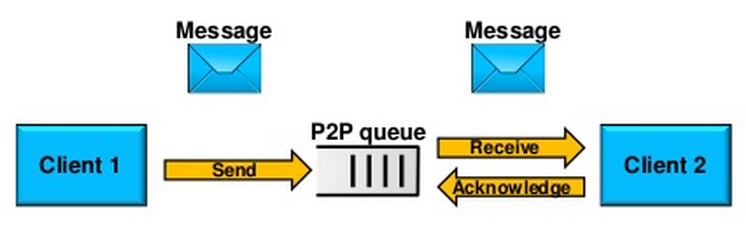
\includegraphics[scale=0.55]{img/obr2}
\end{center}
\begin{tikzpicture}[remember picture,overlay]
    \node[xshift=-0.6cm,yshift=-1.3cm] at (current page.north east){%
    
\includegraphics[width=1cm]{img/pozor}};
\end{tikzpicture}
\end{frame}


\begin{frame}[containsverbatim]\frametitle{Messaging domains}
\begin{itemize}
	\item PubSub
      \begin{itemize}
    	\item Publish-Subscribe domain
		\item Multiple publishers/subscribers
		\item Weak timing (no messages delivered before subscription)
		\item Durable subscriptions available (survive reboot)
      \end{itemize}
\end{itemize}
\begin{center}
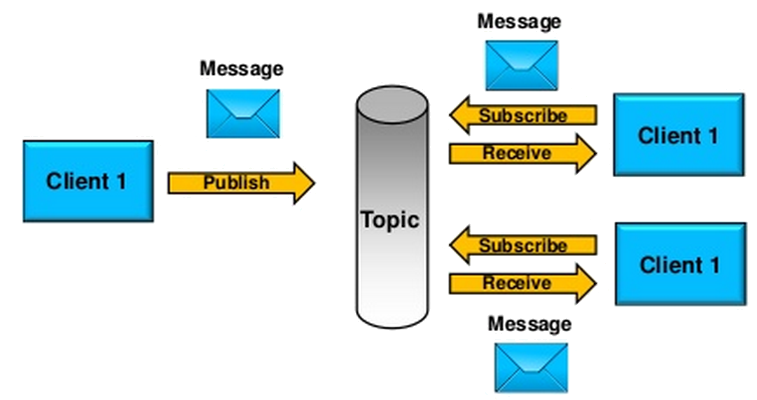
\includegraphics[scale=0.5]{img/obr3_2}
\end{center}
\begin{tikzpicture}[remember picture,overlay]
    \node[xshift=-0.6cm,yshift=-1.3cm] at (current page.north east){%
    
\includegraphics[width=1cm]{img/pozor}};
\end{tikzpicture}
\end{frame}


\begin{frame}[containsverbatim]\frametitle{JMS architecture}
\begin{itemize}
	\item JMS is an interface specification
	  \begin{itemize}
		\item Providers implement queues and topics
	  \end{itemize}
    \item Heavy use of JNDI (Java Naming and Directory Interface)
	  \begin{itemize}
		\item Connection factories (Topic or Queue factory)
		\item Destinations (channels of communication)
	  \end{itemize}
\end{itemize}
\begin{center}
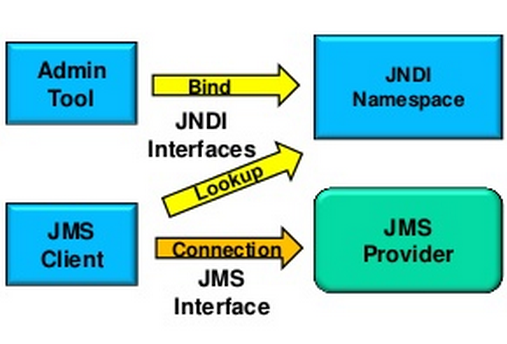
\includegraphics[scale=0.55]{img/obr4}
\end{center}
\end{frame}


\begin{frame}[containsverbatim]\frametitle{JMS programing model}
\begin{center}
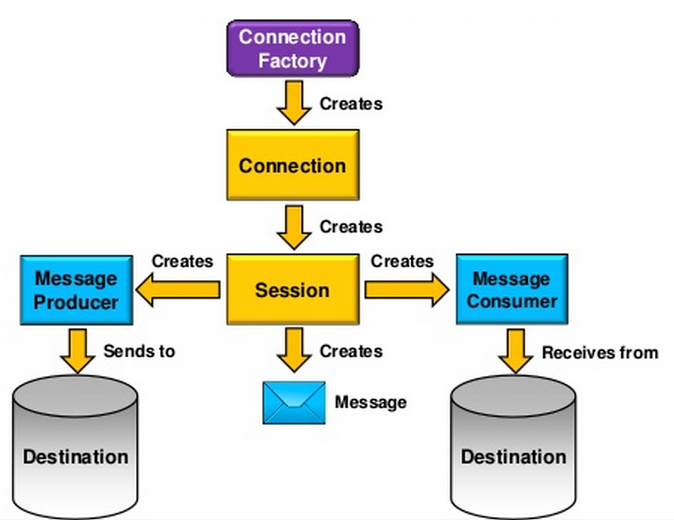
\includegraphics[scale=0.58]{img/obr5}
\end{center}
\begin{tikzpicture}[remember picture,overlay]
    \node[xshift=-0.6cm,yshift=-1.3cm] at (current page.north east){%
    
\includegraphics[width=1cm]{img/pozor}};
\end{tikzpicture}
\end{frame}


\begin{frame}[containsverbatim]\frametitle{JMS programming model}
\begin{itemize}
	\item Connection factory
	  \begin{itemize}
	    \item managed by JMS provider
	    \item \texttt{TopicFactory}
	    \item \texttt{QueueFactory}
	  \end{itemize}
	\item Destination
	  \begin{itemize}
		\item also managed by JMS provider
		\item \texttt{Topic} and \texttt{Queue} channels (and interfaces)
        \item configured on application server (not in application)
	  \end{itemize}
    \item Topic
      \begin{itemize}
    	\item  Many to many (PubSub)
      \end{itemize}
    \item Queue
      \begin{itemize}
    	\item Many to one (P2P)
		\item When message is retrieved, it is deleted from the queue.
      \end{itemize}
\end{itemize}
\begin{tikzpicture}[remember picture,overlay]
    \node[xshift=-0.6cm,yshift=-1.3cm] at (current page.north east){%
    
\includegraphics[width=1cm]{img/pozor}};
\end{tikzpicture}
\end{frame}


\begin{frame}[containsverbatim]\frametitle{JMS model}
\begin{itemize}
	\item Session
	  \begin{itemize}
		\item context to deliver and consume message
		\item created from connections (factories)
		\item lifecycle start and end defined
	  \end{itemize}
    \item Consumer and Producer
	  \begin{itemize}
		\item created by sessions
		\item Session exists for each producer and consumer.
	  \end{itemize}
\end{itemize}
\begin{tikzpicture}[remember picture,overlay]
    \node[xshift=-0.6cm,yshift=-1.3cm] at (current page.north east){%
    
\includegraphics[width=1cm]{img/pozor}};
\end{tikzpicture}
\end{frame}


\begin{frame}[containsverbatim]\frametitle{JMS messages}
\begin{itemize}
  \item \texttt{MapMessage}
	\begin{itemize}
	  \item for sending of key-value pairs
	  \item also sending of objects
      \item[] \vspace*{0.1cm} \begin{footnotesize}
 \begin{verbatim}
MessageProducer producer = session.createProducer(queue);
MapMessage m = session.createMapMessage();
m.setIntProperty("Id", 987654321);
m.setStringProperty("name", "Widget");
m.setDoubleProperty("price", 0.99);
List<String> colors = new ArrayList<String>();
colors.add("red");
colors.add("green");
colors.add("white");
m.setObject("colours", colors);
Producer.send(m);
\end{verbatim}\end{footnotesize}
    \end{itemize}
  \item Consumer receives \texttt{MapMessage} Object
  \item Getters
    \begin{itemize}
      \item \texttt{getInt("key1”)}
	  \item \texttt{getString("key2”)}
	  \item \texttt{getObject("key3”)}
	  \item \texttt{getMapNames()}
    \end{itemize}
\end{itemize}
\begin{tikzpicture}[remember picture,overlay]
    \node[xshift=-0.6cm,yshift=-1.3cm] at (current page.north east){%
    
\includegraphics[width=1cm]{img/oko}};
\end{tikzpicture}
\end{frame}


\begin{frame}[containsverbatim]\frametitle{JMS messages}
\begin{itemize}
  \item \texttt{TextMessage}
    \vspace*{0.1cm}
	\begin{itemize}
	  \item simple string messages
   	  \vspace*{0.1cm}
	  \item[] \begin{footnotesize}\begin{verbatim}
queueConnectionFactory = (QueueConnectionFactory)
    jndiContext.lookup("QueueConnectionFactory");
queue = (Queue) jndiContext.lookup("myQueue");
queueConnection = 
    queueConnectionFactory.createQueueConnection();
queueSession = queueConnection.createQueueSession(false, 
    Session.AUTO_ACKNOWLEDGE);
QueueSender queueSender = queueSession.createSender(queue);
TextMessage textMessage = queueSession.createTextMessage();
textMessage.setText("My message”);
queueSender.send(textMessage);
\end{verbatim}\end{footnotesize}
    \vspace*{0.1cm}
    \item Receiver
    \vspace*{0.1cm}
    \item[] \begin{footnotesize}\begin{verbatim}
queueReceiver = queueSession.createReceiver(queue);
textMessage = (TextMessage) queueReceiver.receive();
String message = textMessage.getText();
\end{verbatim}\end{footnotesize} 
  \end{itemize}
\end{itemize}
\end{frame}


\begin{frame}[containsverbatim]\frametitle{JMS messages}
\begin{itemize}
	\item \texttt{ObjectMessage}
	  \begin{itemize}
		\item used to send serializable objects
		\item \texttt{setObject(Serializable Object)}
		\item \texttt{getObject()}
	  \end{itemize}
    \item \texttt{StreamMessage}
	  \begin{itemize}
		\item for sending of binary primitives
		\item \texttt{getABC}, \texttt{setABC}
        \item where ABC is primitive java type (\texttt{Integer}, \texttt{String}, \ldots)
        \item It is possible to read different type than was written (conversion table exists).
        \item \texttt{null} can be dangerous
          \begin{itemize}
              \item Read is treated as calling the primitive's corresponding \texttt{valueOf(String)} with a \texttt{null} value.
              \item \texttt{char} does not support a String conversion, attempting to read a \texttt{null} value as a \texttt{char} must throw a \texttt{NullPointerException}.
          \end{itemize}
	  \end{itemize}
\end{itemize}
\begin{tikzpicture}[remember picture,overlay]
    \node[xshift=-0.6cm,yshift=-1.3cm] at (current page.north east){%
    
\includegraphics[width=1cm]{img/oko}};
\end{tikzpicture}
\end{frame}


\begin{frame}[containsverbatim]\frametitle{JMS messages}
\begin{itemize}
  \item \texttt{BytesMessage}
	\begin{itemize}
	  \item contains stream of uninterpreted bytes
	  \item based on \texttt{DataInputStream} and \texttt{DataOutputStream}
	  \item binary data
	  \item Methods – corresponding read/write calls
        \begin{itemize}
          \item \texttt{writeDouble}
	      \item \texttt{writeBytes}
          \item \texttt{writeUTF}
	      \item \texttt{readDouble}
	      \item \texttt{readBytes}
	      \item \texttt{readUTF}
	      \item \ldots
        \end{itemize}
	\end{itemize}
\end{itemize}
\begin{textblock}{5}(10.9,3.2)
    {\footnotesize Example JMSP2P}
\end{textblock}
\end{frame}


\begin{frame}[containsverbatim]\frametitle{JNDI}
\begin{itemize}
	\item Java Naming and Directory Interface
    \item JMS is tightly coupled to JNDI
	\item Provider
	  \begin{itemize}
		\item Queue name lookups
		\item an instance implementing the JNDI interface specification and services name lookups.
		\item returns answers to name lookup requests.
	  \end{itemize}
    \item Initial context
      \begin{itemize}
    	\item starting point for name lookups
		\item Different providers need to be parametrized with different properties.
      \end{itemize}
\end{itemize}
\begin{tikzpicture}[remember picture,overlay]
    \node[xshift=-0.6cm,yshift=-1.3cm] at (current page.north east){%
    
\includegraphics[width=1cm]{img/oko}};
\end{tikzpicture}
\end{frame}


\begin{frame}[containsverbatim]\frametitle{JNDI}
\begin{itemize}
	\item Association
	  \begin{itemize}
		\item associate name with object (create binding)
	  \end{itemize}
    \item Find
	  \begin{itemize}
		\item locate object specified by the name
	  \end{itemize}
	\item Context
	  \begin{itemize}
	    \item set of bindings to object names
	    \item similar to e. g. filesystem
	  \end{itemize}
    \item Naming system
	  \begin{itemize}
	    \item set of connected contexts
	    \item LDAP (Lightweight Directory Access Protocol)
	  \end{itemize}
    \item Namespace	
      \begin{itemize}
    	\item all names in naming system
		\item for example all DNS names
      \end{itemize}
\end{itemize}
\end{frame}


\begin{frame}[containsverbatim]\frametitle{JNDI architecture}
\begin{itemize}
	\item Defines only interface for client accesses
	\item Common API for service providers
	\item JNDI SPI (service provider interface) allows to use different naming service providers
	\item Custom naming service may be developed by implementing JNDI SPI
\end{itemize}
\begin{center}
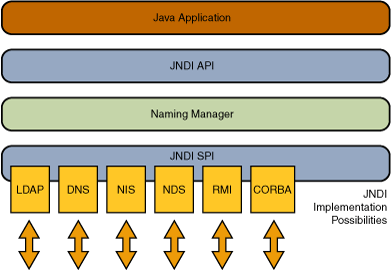
\includegraphics[scale=0.77]{img/obr6}
\end{center}
\begin{tikzpicture}[remember picture,overlay]
    \node[xshift=-0.6cm,yshift=-1.3cm] at (current page.north east){%
    
\includegraphics[width=1cm]{img/oko}};
\end{tikzpicture}
\end{frame}


\begin{frame}[containsverbatim]\frametitle{JNDI services}
\begin{itemize}
	\item Access to directory services through common API
	\item Directories are structured trees of informations
	\item Directory services
    \begin{itemize}
    	\item LDAP (Lightweight Directory Access Protocol)
    	\item DNS
    	\item NIS (Network Information Service) (Oracle)
    	\item NetWare Directory Services (NDS)
		\item Microsoft Active Directory
		\item IBM Lotus Notes/Domino
		\item Common Object Request Broker Architecture (CORBA)
    \end{itemize}
\end{itemize}
\end{frame}

\begin{frame}[containsverbatim]\frametitle{Message consumptions}
\begin{itemize}
	\item Asynchronous
	  \begin{itemize}
		\item A client can register a \textit{message listener} with a consumer.
		\item Whenever a message arrives at the destination, the JMS provider delivers the message by calling the listener's \texttt{onMessage()} method.
	  \end{itemize}
    \item Synchronous
      \begin{itemize}
 	   \item A subscriber or a receiver explicitly fetches the message from the destination by calling the \texttt{receive} method.
		\item The \texttt{receive} method can \textit{block} until a message arrives or can time out if a message does not arrive within a specified time limit.
      \end{itemize}
\end{itemize}
\begin{textblock}{5}(8.9,3.4)
    {\footnotesize Examples jms-chat, JMSChat}
\end{textblock}
\begin{tikzpicture}[remember picture,overlay]
    \node[xshift=-0.6cm,yshift=-1.3cm] at (current page.north east){%
    
\includegraphics[width=1cm]{img/pozor}};
\end{tikzpicture}
\end{frame}


\begin{frame}[containsverbatim]\frametitle{JMS features}
\begin{itemize}
	\item Additional features turned off by default
	\item Message acknowledgement
	\item Message priorities
	\item Persistent delivery mode
	\item Control of message expiration
	\item Durable subscriptions
	\item Message transactions
\end{itemize}
\end{frame}


\begin{frame}[containsverbatim]\frametitle{Message acknowledgements}
\begin{itemize}
  \item In non-transacted sessions
	\begin{itemize}
	  \item client receives the message
	  \item message is processed
	  \item acknowledgement is sent
	\end{itemize}
  \item Acknowledgement modes
	\begin{itemize}
	  \item Auto-acknowledgement
        \begin{itemize}
          \item An acknowledgement is sent after a successful return from \texttt{receive} function, or when listener successfully returns.
          \item \texttt{Session.AUTO\_ACKNOWLEDGE}
        \end{itemize}
	  \item Client acknowledgement 
        \begin{itemize}
          \item Explicit call of message's \texttt{acknowledge} method.
	      \item \texttt{Session.CLIENT\_ACKNOWLEDGE}
        \end{itemize}
      \item Lazy client acknowledgement 
        \begin{itemize}
          \item reduces JMS overhead
          \item acknowledgment each time it has received a fixed number of messages, or when a fixed time interval has elapsed since the last acknowledgment (10 messages and 7 seconds)
          \item Broker does not acknowledge receipt of the client acknowledgment.
          \item You have no way to confirm that your acknowledgment has been received; if it is lost in transmission, the broker may redeliver the same message more than once, so duplicates may occur.
	      \item \texttt{Session.DUPS\_OK\_ACKNOWLEDGE}
        \end{itemize}
    \end{itemize}
\end{itemize}
\begin{tikzpicture}[remember picture,overlay]
    \node[xshift=-0.6cm,yshift=-1.3cm] at (current page.north east){%
    
\includegraphics[width=1cm]{img/pozor}};
\end{tikzpicture}
\end{frame}


\begin{frame}[containsverbatim]\frametitle{Persistent delivery mode}
\begin{itemize}
    \item Persistent delivery mode
      \begin{itemize}
        \item default mode
        \item A message sent with this delivery mode is logged to stable storage when it is sent.
    	\item Messages can survive provider crashes.
	    \item Persistent delivery needs more performance.
    	\item Persistent delivery needs more storage.
      \end{itemize}
	\item Non persistent delivery mode
	  \begin{itemize}
	      \item does not require the JMS provider to store the message or otherwise guarantee that it is not lost if the provider fails
	      \item may improve performance, but you should use it only if your application can afford to miss messages.
	      \item Can be enabled using: \texttt{producer.setDeliveryMode(DeliveryMode.NON\_PERSISTENT);}
	  \end{itemize}
\end{itemize}
\end{frame}


\begin{frame}[containsverbatim]\frametitle{Priorities, expirations}
\begin{itemize}
	\item Priorities
      \begin{itemize}
    	\item 10 levels
		\item 0 – lowest priority
		\item 4 – default priority
		\item 9 – highest priority
		\item Queues and Topics may grow big
		\item \texttt{producer.setPriority(7);}
      \end{itemize}
    \item Expiration
	  \begin{itemize}
		\item By default, messages never expire.
		\item Expiration may be useful when using priorities.
		\item TTL may be set to every message in milliseconds.
		\item \texttt{producer.setTimeToLive(10000);}
	  \end{itemize}
	\item {\small \texttt{topicPublisher.publish(message,  }}
	\item[] {\small \texttt{ ~ ~DeliveryMode.NON\_PERSISTENT, 8, 10000);}}
\end{itemize}
\begin{tikzpicture}[remember picture,overlay]
    \node[xshift=-0.6cm,yshift=-1.3cm] at (current page.north east){%
    
\includegraphics[width=1cm]{img/oko}};
\end{tikzpicture}
\end{frame}


\begin{frame}[containsverbatim]\frametitle{Durable subscriptions, transactions}
\begin{itemize}
	\item Default subscriptions are non-persistent
	  \begin{itemize}
		\item After each reboot the receiver must subscribe again.
		\item Messages that arrived during the reboot will not be delivered.
	  \end{itemize}
    \item Durable subscriptions are persistent
	  \begin{itemize}
		\item After reboot the receiver do not need to subscribe again.
		\item Messages that arrived during reboot will be delivered after a~new session is created.
	  \end{itemize}
    \item Subscription is not session
	  \begin{itemize}
		\item In first case, messages M3 And M4 are not delivered.
        \item In second case, messages M2, M4, M5 are received when user starts new session.
	  \end{itemize}
\end{itemize}
\begin{center}
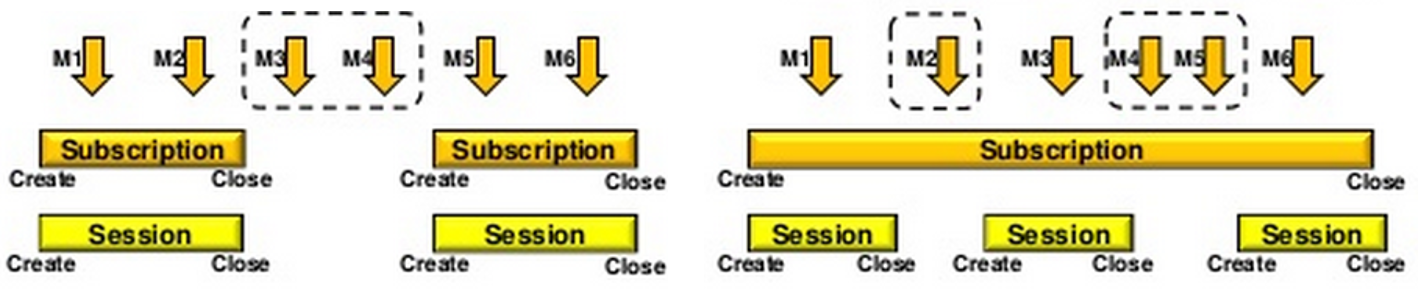
\includegraphics[scale=0.31]{img/obr7}
\end{center}
\begin{tikzpicture}[remember picture,overlay]
    \node[xshift=-0.6cm,yshift=-1.3cm] at (current page.north east){%
    
\includegraphics[width=1cm]{img/lupa}};
\end{tikzpicture}
\end{frame}


\begin{frame}[containsverbatim]\frametitle{Transactions}
\begin{itemize}
	\item Transactions allows grouping of operations into an atomic unit of work.
	\item During rollback all produced messages are destroyed, consumed messages are recovered.
	\item Commit means that all messages are sent and consumed messages acknowledged.
	\item Transactions cannot be combined with request-reply mechanism.
\end{itemize}
\begin{center}
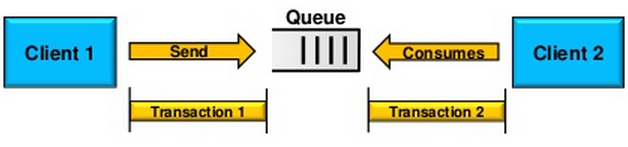
\includegraphics[scale=0.69]{img/obr8}
\end{center}
\begin{tikzpicture}[remember picture,overlay]
    \node[xshift=-0.6cm,yshift=-1.3cm] at (current page.north east){%
    
\includegraphics[width=1cm]{img/zarovka}};
\end{tikzpicture}
\end{frame}


\begin{frame}[containsverbatim]\frametitle{Transactions}
\begin{itemize}
  \item Rollback
    \begin{itemize}
	  \item After rollback, all “buffered” messages are destroyed.
    \end{itemize}
  \item Commit
    \begin{itemize}
      \item After commit, messages begins to be retrieved.
    \end{itemize}
\end{itemize}
\begin{center}
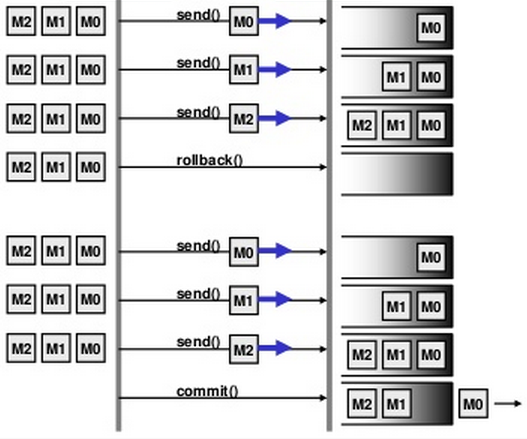
\includegraphics[scale=0.57]{img/obr9}
\end{center}
\end{frame}


\begin{frame}[containsverbatim]\frametitle{ActiveMQ}
\begin{itemize}
    \item How to run the broker:
      \begin{enumerate}
          \item Download the distribution package from \url{https://activemq.apache.org/components/classic/download/} or from \url{https://activemq.apache.org/components/artemis/download/}
          \item Run the broker (you can use command \texttt{./activemq start} in the \texttt{bin} directory in Linux or \texttt{./artemis create ../../testArtemis} and then \texttt{./artemis run} in the \texttt{testArtemis} directory)
      \end{enumerate}
    \item Default URL of the broker is \texttt{ActiveMQConnection.DEFAULT\_BROKER\_URL;}
    or \texttt{DefaultConnectionProperties.DEFAULT\_BROKER\_URL;}
\end{itemize}
\begin{textblock}{5}(9.9,4.6)
    {\footnotesize Example jms-chat-amq}
\end{textblock}
\end{frame}

\begin{frame}[containsverbatim]\frametitle{References}
\begin{itemize}
    \item JMS Concepts
	  \begin{itemize}
		\item \url{https://docs.oracle.com/javaee/7/tutorial/jms-concepts.htm}
	  \end{itemize}
    \item JMS Examples
	  \begin{itemize}
		\item \url{https://docs.oracle.com/javaee/7/tutorial/jms-examples.htm}
	  \end{itemize}
	\item Tutorial
	  \begin{itemize}
	      \item \url{https://www.javatpoint.com/jms-tutorial}
	  \end{itemize}
	\item ActiveMQ
	  \begin{itemize}
	    \item \url{https://activemq.apache.org/}
	    \item \url{https://examples.javacodegeeks.com/enterprise-java/jms/apache-activemq-hello-world-example/}
	  \end{itemize}
   \item Examples
     \begin{itemize}
         \item \url{https://hantsy.medium.com/kickstart-a-jakarta-ee-10-application-d579577af634}
     \end{itemize}
\end{itemize}
\end{frame}

\bluepage{Thank you for your attention!}


\end{document}
